\documentclass[11pt]{amsart}
\usepackage{geometry}                % See geometry.pdf to learn the layout options. There are lots.
\geometry{letterpaper}                   % ... or a4paper or a5paper or ... 
%\geometry{landscape}                % Activate for for rotated page geometry
%\usepackage[parfill]{parskip}    % Activate to begin paragraphs with an empty line rather than an indent
\usepackage{graphicx}
\usepackage{amssymb}
\usepackage{epstopdf}
\usepackage{multicol}
\DeclareGraphicsRule{.tif}{png}{.png}{`convert #1 `dirname #1`/`basename #1 .tif`.png}
\usepackage{/Library/Frameworks/R.framework/Resources/share/texmf/Sweave}

\title{Genotypic variation influences lichen co-occurrence network structure}
\author{M.K. Lau, L.J. Lamit, T.G. Whitham}
%\date{}                                           % Activate to display a given date or no date

\begin{document}
\maketitle

\section{Things to Do}
\begin{enumerate}
\item Do a whole network analysis using PerMANOVA
\item Can we do pathway de-proliferation?
\item Use eigenvector centrality. What is the dominant eigenvalue for each matrix?
\item Use Fath and Patten's 1998 network mutualism in utility analysis
\item Fix the gplot inputs for genotype vertex attributes (it is
  currently using the tree level data)
\item
\item
\end{enumerate}

\section{Generate lichen network models for all genotypes in each garden}

\subsection{Load packages}

\begin{Schunk}
\begin{Sinput}
> require(RLRsim)
> require(lme4)
> require(sna)
\end{Sinput}
\begin{Soutput}
     Tools for Social Network Analysis
Version      2.2-0 created on      2010-11-21.
copyright (c) 2005, Carter T. Butts, University of California-Irvine
Type help(package="sna") to get started.
\end{Soutput}
\begin{Sinput}
> require(vegan)
> require(xtable)
> require(gplots)
\end{Sinput}
\begin{Soutput}
gdata: read.xls support for 'XLS' (Excel 97-2004) files ENABLED.

gdata: read.xls support for 'XLSX' (Excel 2007+) files ENABLED.
\end{Soutput}
\begin{Sinput}
> source("source/CorNets.R")
> source("source/pairs.R")
> se = function(x) {
+     sd(x)/sqrt(length(x))
+ }
> binary = function(x, bin = 0) {
+     x[x > bin] = 1
+     return(x)
+ }
> richness = function(x) {
+     x = apply(x, 2, sum)
+     x[x != 0] = 1
+     sum(x)
+ }
> bplot = function(x, y, ylab = "") {
+     mu. = tapply(y, x, mean)
+     se. = tapply(y, x, se)
+     barplot2(mu., plot.ci = TRUE, ci.u = mu. + se., ci.l = mu. - 
+         se., las = 2, ylab = ylab)
+ }
> which.garden = function(x) {
+     x = unlist(strsplit(as.character(x), split = ".", fixed = TRUE))[1]
+     x = unlist(strsplit(x, split = ""))
+     if (length(x) < 3) {
+         x = "ONC"
+     }
+     else {
+         x = "PIT"
+     }
+     return(x)
+ }
> lco2quad = function(x) {
+     com = x[, -1:-6]
+     com = apply(com, 1, sum)
+     x = x[, 5:6]
+     out = array(0, dim = c(max(x), max(x)))
+     for (i in (1:nrow(x))) {
+         out[x[i, 1], x[i, 2]] = com[i]
+     }
+     return(out)
+ }
> exp.m <- function(mat, n) {
+     if (n == 1) 
+         return(mat)
+     result <- diag(1, ncol(mat))
+     while (n > 0) {
+         if (n%%2 != 0) {
+             result <- result %*% mat
+             n <- n - 1
+         }
+         mat <- mat %*% mat
+         n <- n/2
+     }
+     return(result)
+ }
> proliferate = function(g = "graph", lim = 10000) {
+     n = numeric()
+     for (i in 1:lim) {
+         n[i] = sum(exp.m(g, i))
+         if (n[i] == Inf) {
+             break
+         }
+     }
+     n = n[-i]
+     return(n)
+ }
\end{Sinput}
\end{Schunk}

\subsection{Data Summary}
NOTE: there was a data entry error for tree N4.30, changed 11 to 1 in LCO\_data\_ONC\_PIT.csv.

\begin{Schunk}
\begin{Sinput}
> lco = read.csv("data/LCO_data_ONC_PIT.csv")
\end{Sinput}
\end{Schunk}


\begin{Schunk}
\begin{Sinput}
> xtable(summary(lco[, 1:6]), table.placement = "tbp")
\end{Sinput}
% latex table generated in R 2.12.1 by xtable 1.5-6 package
% Tue Jul 26 16:50:34 2011
\begin{table}[ht]
\begin{center}
\begin{tabular}{rllllll}
  \hline
 &      Tree &      Geno &      Year &   Quadrat &      Row &      Col \\ 
  \hline
1 & N1.10  : 100   & 996    :1000   & Min.   :2010   & n45.55:4850   & Min.   : 1.0   & Min.   : 1.0   \\ 
  2 & N1.11  : 100   & 1008   : 900   & 1st Qu.:2011   & n80.90:3050   & 1st Qu.: 3.0   & 1st Qu.: 3.0   \\ 
  3 & N1.24  : 100   & 1017   : 750   & Median :2011   &  & Median : 5.5   & Median : 5.5   \\ 
  4 & N1.27  : 100   & 11     : 700   & Mean   :2011   &  & Mean   : 5.5   & Mean   : 5.5   \\ 
  5 & N1.28  : 100   & 10     : 600   & 3rd Qu.:2011   &  & 3rd Qu.: 8.0   & 3rd Qu.: 8.0   \\ 
  6 & N1.31  : 100   & 1023   : 600   & Max.   :2011   &  & Max.   :10.0   & Max.   :10.0   \\ 
  7 & (Other):7300   & (Other):3350   &  &  &  &  \\ 
   \hline
\end{tabular}
\end{center}
\end{table}\end{Schunk}

\begin{Schunk}
\begin{Sinput}
> xtable(summary(lco[, 7:10]), table.placement = "tbp")
\end{Sinput}
% latex table generated in R 2.12.1 by xtable 1.5-6 package
% Tue Jul 26 16:50:34 2011
\begin{table}[ht]
\begin{center}
\begin{tabular}{rllll}
  \hline
 &      Xgal &      Csub &      Lsp &      Chol \\ 
  \hline
1 & Min.   :0.0000   & Min.   :0.00000   & Min.   :0.00000   & Min.   :0.000000   \\ 
  2 & 1st Qu.:0.0000   & 1st Qu.:0.00000   & 1st Qu.:0.00000   & 1st Qu.:0.000000   \\ 
  3 & Median :1.0000   & Median :0.00000   & Median :0.00000   & Median :0.000000   \\ 
  4 & Mean   :0.5084   & Mean   :0.09165   & Mean   :0.02076   & Mean   :0.009494   \\ 
  5 & 3rd Qu.:1.0000   & 3rd Qu.:0.00000   & 3rd Qu.:0.00000   & 3rd Qu.:0.000000   \\ 
  6 & Max.   :1.0000   & Max.   :1.00000   & Max.   :1.00000   & Max.   :1.000000   \\ 
   \hline
\end{tabular}
\end{center}
\end{table}\end{Schunk}

\begin{Schunk}
\begin{Sinput}
> xtable(summary(lco[, 13:ncol(lco)]), table.placement = "tbp")
\end{Sinput}
% latex table generated in R 2.12.1 by xtable 1.5-6 package
% Tue Jul 26 16:50:34 2011
\begin{table}[ht]
\begin{center}
\begin{tabular}{rlll}
  \hline
 &      Pads &      Pund &      Rsp \\ 
  \hline
1 & Min.   :0.000000   & Min.   :0.000000   & Min.   :0.000000   \\ 
  2 & 1st Qu.:0.000000   & 1st Qu.:0.000000   & 1st Qu.:0.000000   \\ 
  3 & Median :0.000000   & Median :0.000000   & Median :0.000000   \\ 
  4 & Mean   :0.002532   & Mean   :0.002025   & Mean   :0.002532   \\ 
  5 & 3rd Qu.:0.000000   & 3rd Qu.:0.000000   & 3rd Qu.:0.000000   \\ 
  6 & Max.   :1.000000   & Max.   :1.000000   & Max.   :1.000000   \\ 
   \hline
\end{tabular}
\end{center}
\end{table}\end{Schunk}

\subsection{Separate Community Matrixes by Tree}
\begin{Schunk}
\begin{Sinput}
> lco = lco[lco$Quadrat == "n45.55", ]
> lco.l = list()
> tree.names = as.character(unique(lco$Tree))
\end{Sinput}
\end{Schunk}

\begin{Schunk}
\begin{Sinput}
> for (i in (1:length(tree.names))) {
+     lco.l[[i]] = lco[lco$Tree == tree.names[i], ]
+ }
> names(lco.l) = tree.names
> any(table(tree.names) != 1)
\end{Sinput}
\begin{Soutput}
[1] FALSE
\end{Soutput}
\end{Schunk}

\subsection{Separate garden, genotype and community data}
\begin{Schunk}
\begin{Sinput}
> garden = sapply(tree.names, which.garden)
> geno = unlist(lapply(lco.l, function(x) as.character(x$Geno[1])))
> com.l = lapply(lco.l, function(x) x[, (1:ncol(x))[colnames(x) == 
+     "Xgal"]:ncol(x)])
\end{Sinput}
\end{Schunk}

\begin{Schunk}
\begin{Sinput}
> geno.table = tapply(factor(geno), garden, table)
> geno.table = rbind(geno.table$ONC, geno.table$PIT)
> rownames(geno.table) = c("ONC", "PIT")
> geno.table = geno.table[, order(apply(geno.table, 2, sum), decreasing = TRUE)]
> xtable(geno.table)
\end{Sinput}
% latex table generated in R 2.12.1 by xtable 1.5-6 package
% Tue Jul 26 16:50:34 2011
\begin{table}[ht]
\begin{center}
\begin{tabular}{rrrrrrrrrrrrrrr}
  \hline
 & 996 & 1008 & 1017 & 11 & 10 & 1023 & 1007 & 999 & T6 & 1012 & 1005 & WC5 & H10 & RL6 \\ 
  \hline
ONC &   8 &   8 &   6 &   5 &   4 &   4 &   4 &   3 &   3 &   4 &   4 &   4 &   3 &   3 \\ 
  PIT &   4 &   3 &   3 &   4 &   4 &   4 &   3 &   4 &   4 &   1 &   0 &   0 &   0 &   0 \\ 
   \hline
\end{tabular}
\end{center}
\end{table}\begin{Sinput}
> barplot(geno.table, beside = FALSE, las = 2, ylab = "Number of Trees", 
+     col = c(1, 0))
> legend("topright", c("ONC", "PIT"), fill = c(1, 0), bty = "n")
\end{Sinput}
\end{Schunk}
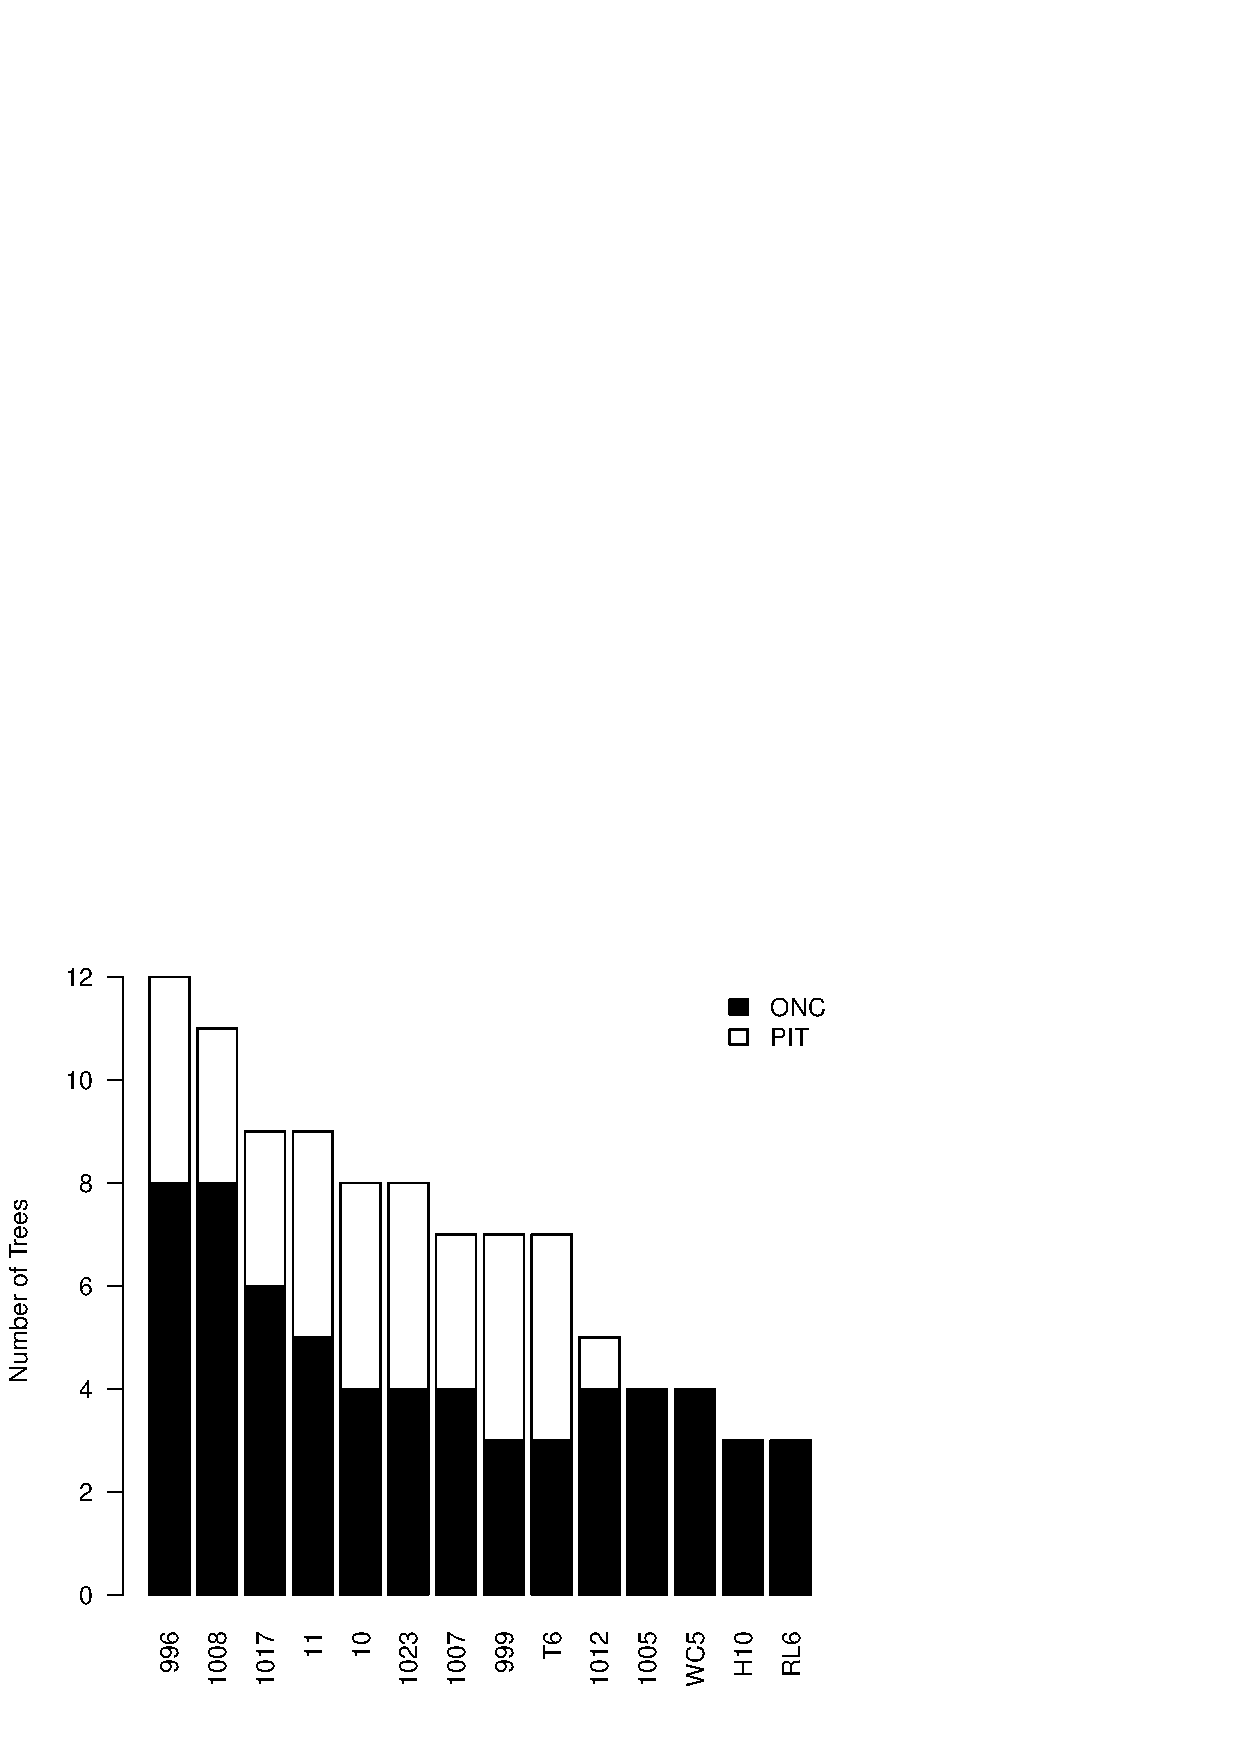
\includegraphics{LCO_analyses-009}

\subsection{Convert to Quadrat View}

\begin{Schunk}
\begin{Sinput}
> quad.l = lapply(lco.l, lco2quad)
\end{Sinput}
\end{Schunk}

\paragraph{}Using the \texttt{kendall.pairs} function at an $\alpha$
level of 0.05 and adjusting for multiple tests, we can model each
community network using the pairwise correlations of all species pairs.

\begin{Schunk}
\begin{Sinput}
> zero.na = function(x) {
+     x[is.na(x)] = 0
+     return(x)
+ }
> cor.l = lapply(com.l, kendall.pairs, alpha = 0.05, p.adj = TRUE)
> cor.l = lapply(cor.l, zero.na)
\end{Sinput}
\end{Schunk}

\section{Network Statistics}

\begin{Schunk}
\begin{Sinput}
> A = lapply(com.l, function(x) apply(x, 2, sum))
> A. = lapply(A, binary)
> R = unlist(lapply(com.l, richness))
> n = unlist(lapply(cor.l, function(x) length(apply(x, 1, sum)[abs(apply(x, 
+     1, sum)) > 0])))
> L = unlist(lapply(cor.l, function(x) length(x[x != 0])/2))
> C = L/(n * (n - 1))
> C[is.na(C)] = 0
> abs.cor.l = lapply(cor.l, abs)
> C.f = unlist(lapply(abs.cor.l, function(x) centralization(x, 
+     degree, mode = "graph")))
\end{Sinput}
\end{Schunk}

%% \subsection{ANOVA}

%% <<>>=
%%   aov.n = aov(sqrt(n)~factor(geno)*factor(garden))
%%   aov.L = aov(sqrt(L)~factor(geno)*factor(garden))
%%   aov.C = aov(C~factor(geno)*factor(garden))
%%   aov.Cf = aov(C.f~factor(geno)*factor(garden))

%%   aov.list = list(aov.n,aov.L,aov.C,aov.Cf)
%% @ 

%% <<results=tex>>=
%%   for (i in (1:length(aov.list))){
%%   print(xtable(summary(aov.list[[i]])))
%%   }
%% @ 


%% <<>>=
%% shapiro.test(residuals(aov.n))
%% shapiro.test(residuals(aov.L))
%% shapiro.test(residuals(aov.C))

%% shapiro.test(n)
%% shapiro.test(L)
%% shapiro.test(C)

%% hist(residuals(aov.n))
%% hist(residuals(aov.L))
%% hist(residuals(aov.C))

%% qqnorm(residuals(aov.C))

%% hist(residuals(aov.n))
%% hist(residuals(aov.L))
%% hist(residuals(aov.C))

%% fligner.test(n~factor(geno))
%% fligner.test(L~factor(geno))
%% fligner.test(C~factor(geno))
%% @ 

\begin{Schunk}
\begin{Sinput}
> input.pairs = cbind(R, n, L, C, C.f)
> pairs.onc = input.pairs[garden == "ONC", ]
> pairs.pit = input.pairs[garden == "PIT", ]
\end{Sinput}
\end{Schunk}

\begin{Schunk}
\begin{Sinput}
> pairs(input.pairs, upper.panel = panel.lm, lower.panel = panel.cor)
\end{Sinput}
\end{Schunk}
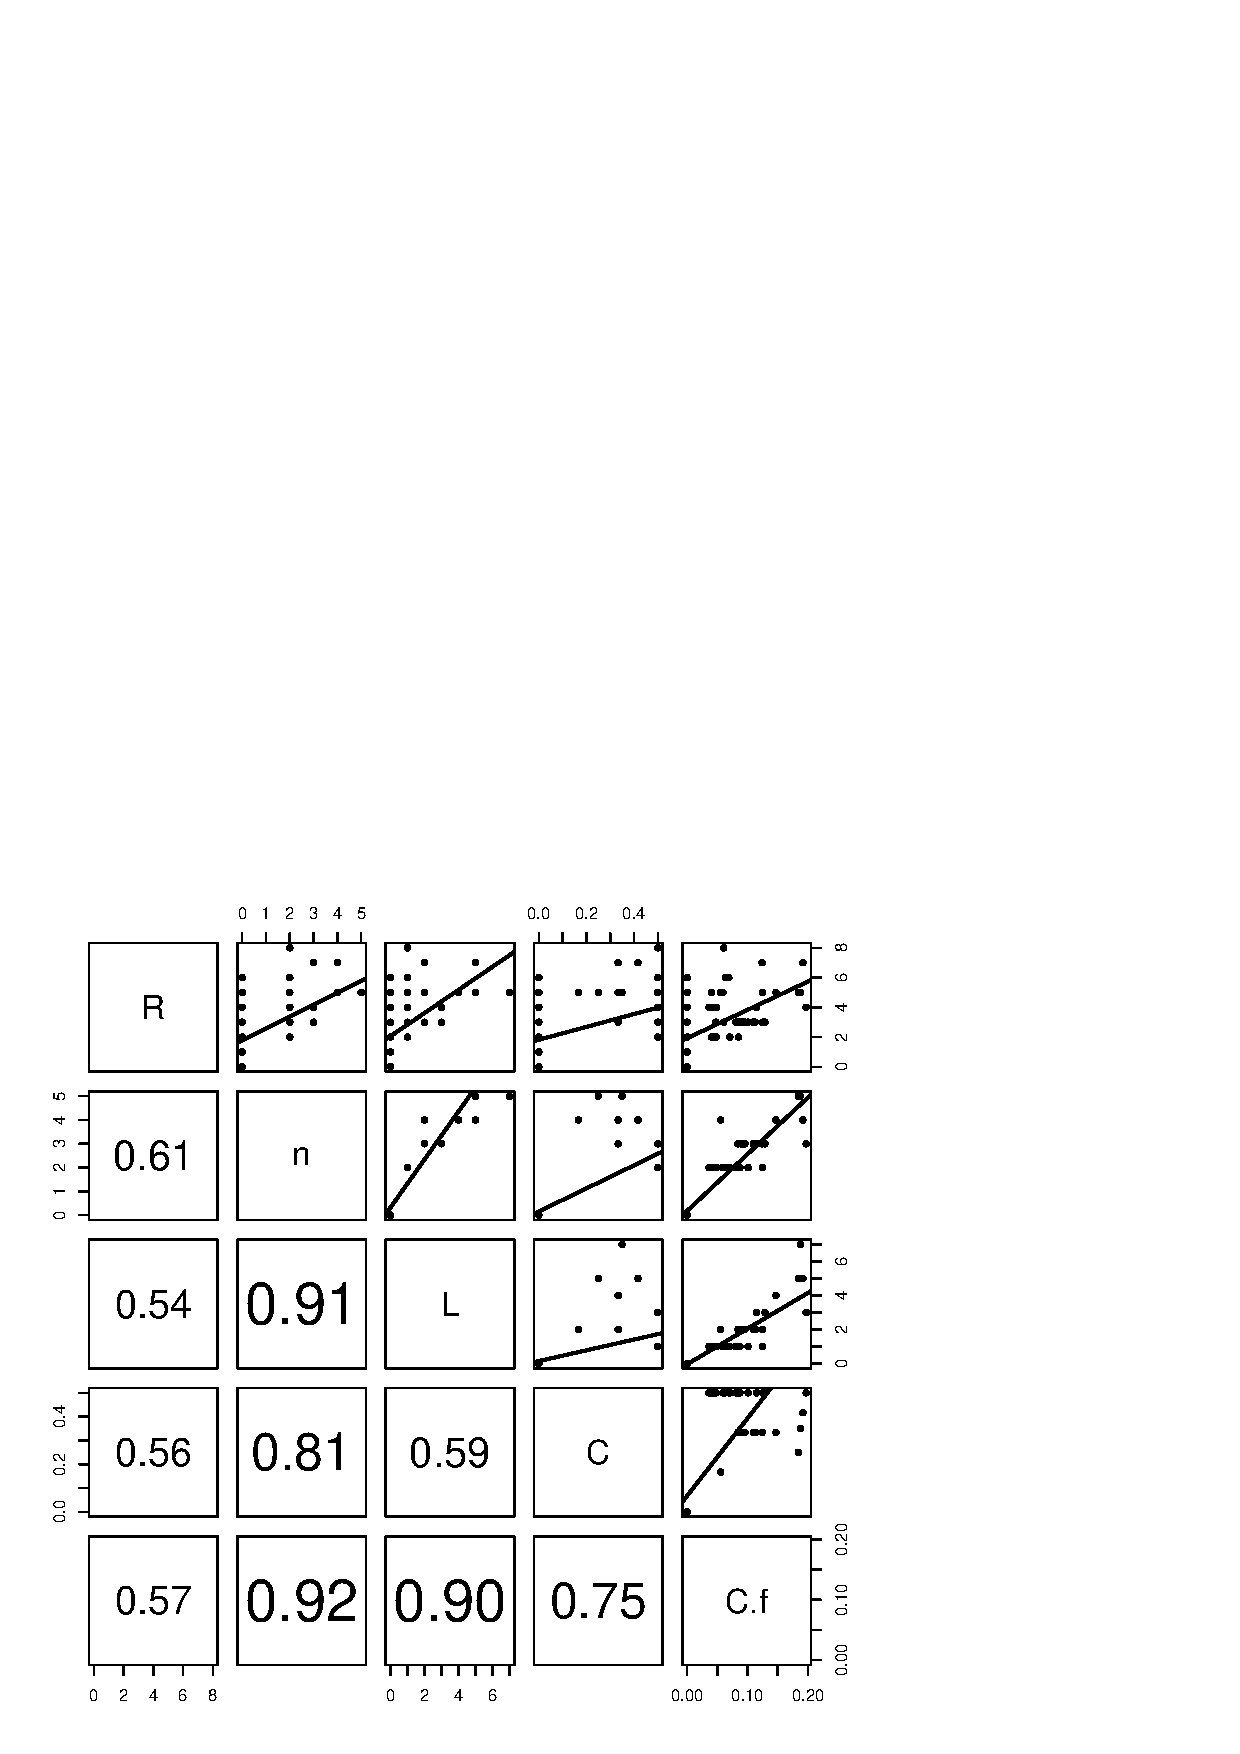
\includegraphics{LCO_analyses-014}

\begin{Schunk}
\begin{Sinput}
> pairs(pairs.onc, upper.panel = panel.lm, lower.panel = panel.cor)
\end{Sinput}
\end{Schunk}
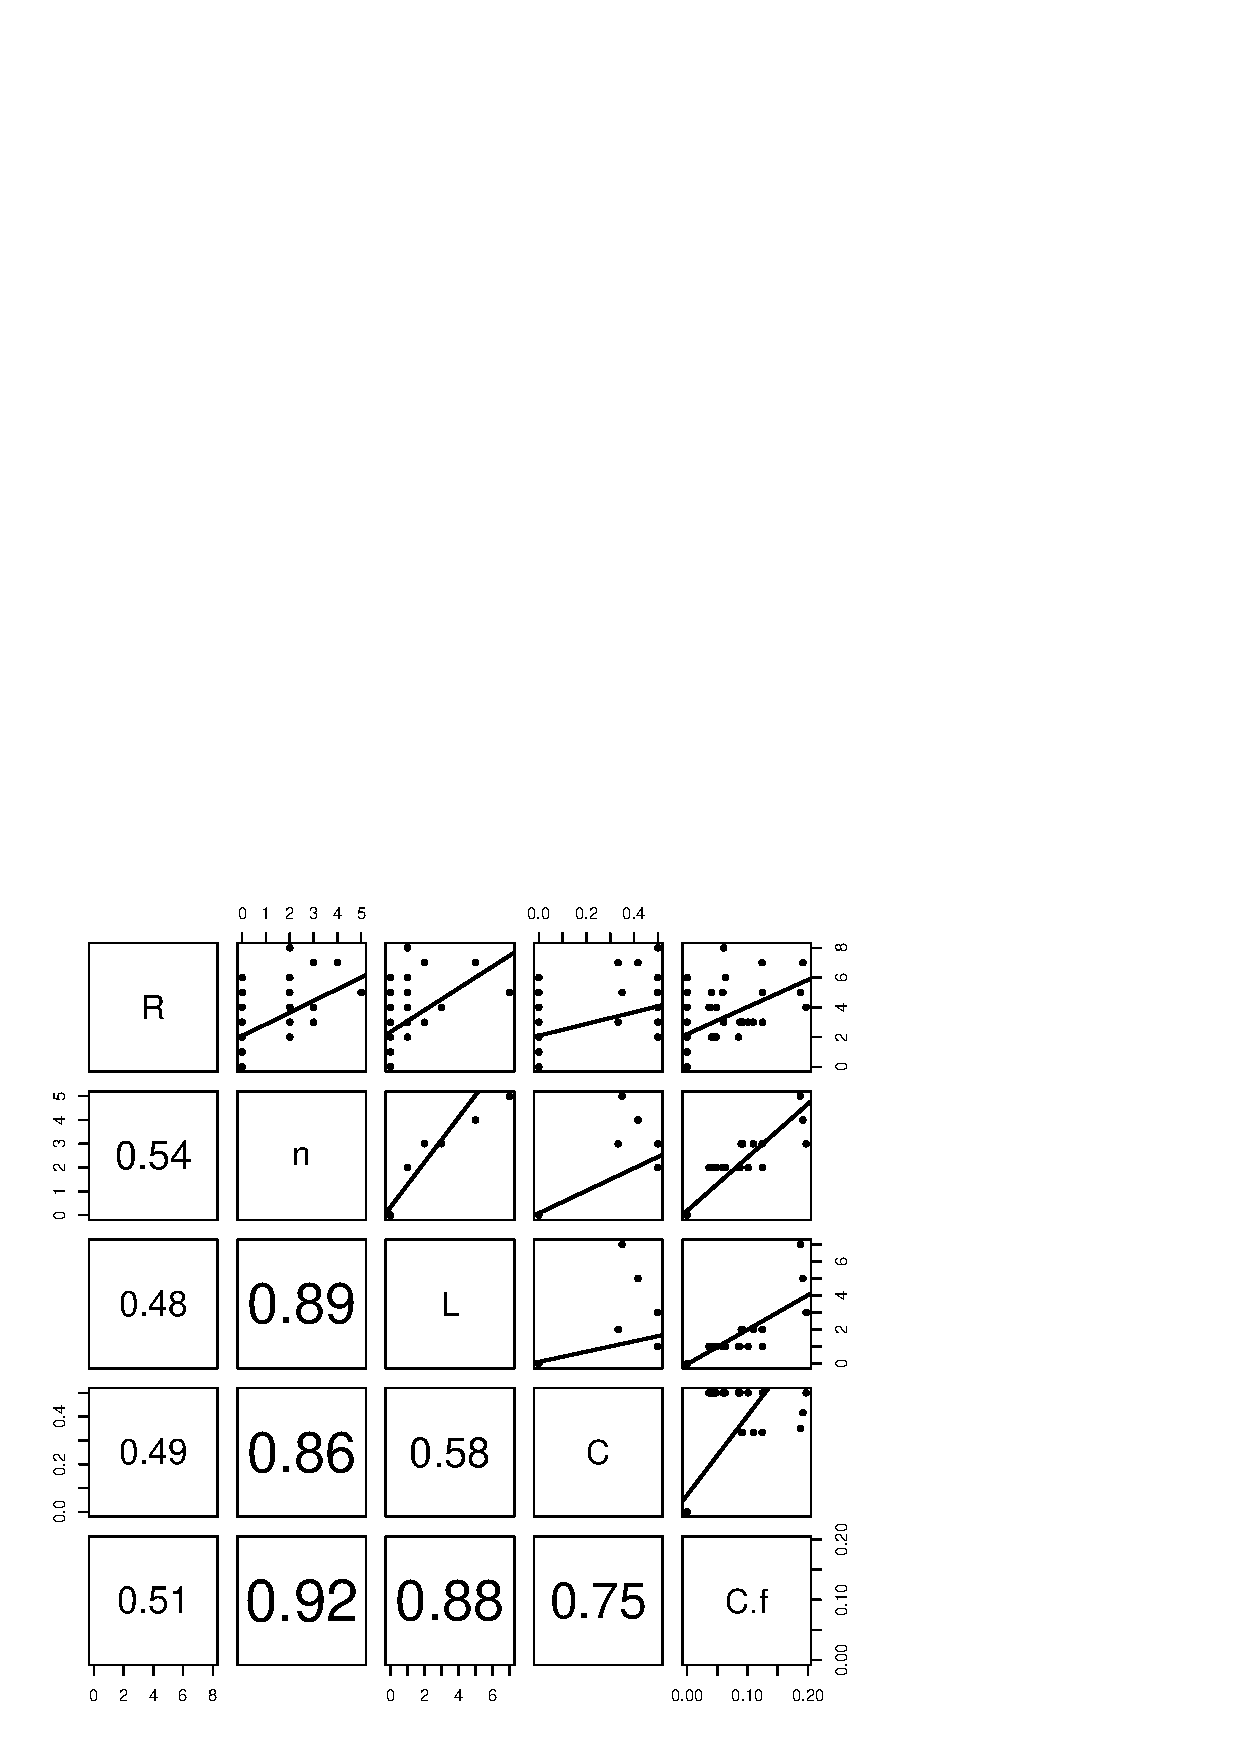
\includegraphics{LCO_analyses-015}

\begin{Schunk}
\begin{Sinput}
> pairs(pairs.pit, upper.panel = panel.lm, lower.panel = panel.cor)
\end{Sinput}
\end{Schunk}
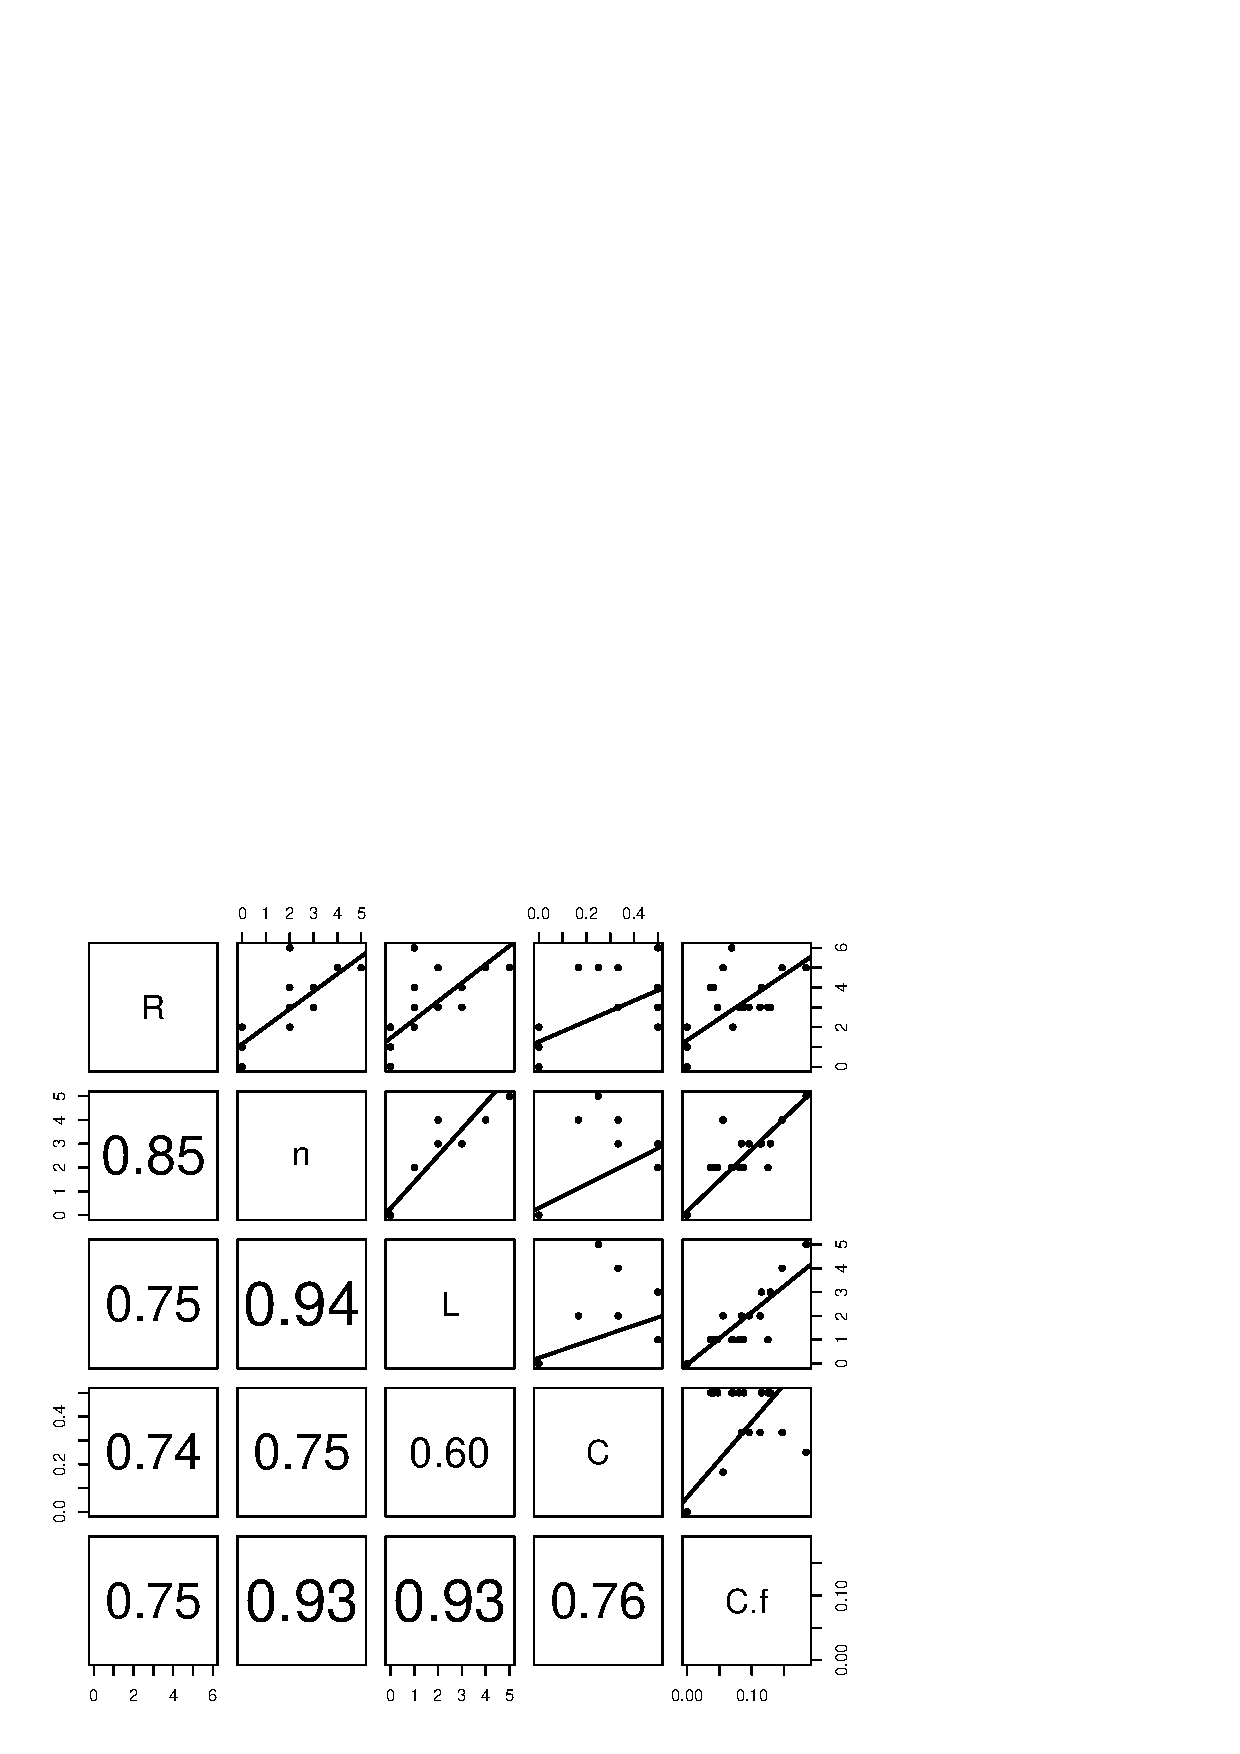
\includegraphics{LCO_analyses-016}

\subsection{REML}
\paragraph{}Separate the analysis of ONC and PIT due to unequal
representation of genotypes at both gardens. 

\begin{Schunk}
\begin{Sinput}
> geno.onc = geno[garden == "ONC"]
> n.onc = n[garden == "ONC"]
> log.n.onc = log(n.onc + 0.5)
> L.onc = L[garden == "ONC"]
> log.L.onc = log(L.onc + 0.5)
> C.onc = C[garden == "ONC"]
> Cf.onc = C.f[garden == "ONC"]
> asin.sqrt.CF.onc = asin(sqrt(Cf.onc))
> exactRLRT(lmer(n.onc ~ 1 | geno.onc))
\end{Sinput}
	simulated finite sample distribution of RLRT.  (p-value based on 10000
	simulated values)

data:  
RLRT = 3.151, p-value = 0.0325\begin{Sinput}
> exactRLRT(lmer(log.n.onc ~ 1 | geno.onc))
\end{Sinput}
	simulated finite sample distribution of RLRT.  (p-value based on 10000
	simulated values)

data:  
RLRT = 4.9866, p-value = 0.0099\begin{Sinput}
> exactRLRT(lmer(L.onc ~ 1 | geno.onc))
\end{Sinput}
	simulated finite sample distribution of RLRT.  (p-value based on 10000
	simulated values)

data:  
RLRT = 0, p-value = 0.4589\begin{Sinput}
> exactRLRT(lmer(log.L.onc ~ 1 | geno.onc))
\end{Sinput}
	simulated finite sample distribution of RLRT.  (p-value based on 10000
	simulated values)

data:  
RLRT = 3.3797, p-value = 0.0287\begin{Sinput}
> exactRLRT(lmer(C.onc ~ 1 | geno.onc))
\end{Sinput}
	simulated finite sample distribution of RLRT.  (p-value based on 10000
	simulated values)

data:  
RLRT = 7.0159, p-value = 0.0038\begin{Sinput}
> exactRLRT(lmer(Cf.onc ~ 1 | geno.onc))
\end{Sinput}
	simulated finite sample distribution of RLRT.  (p-value based on 10000
	simulated values)

data:  
RLRT = 0.8348, p-value = 0.16\begin{Sinput}
> exactRLRT(lmer(asin.sqrt.CF.onc ~ 1 | geno.onc))
\end{Sinput}
	simulated finite sample distribution of RLRT.  (p-value based on 10000
	simulated values)

data:  
RLRT = 2.8031, p-value = 0.0423\begin{Sinput}
> geno.pit = geno[garden == "PIT"]
> n.pit = n[garden == "PIT"]
> log.n.pit = log(n.pit + 0.5)
> L.pit = L[garden == "PIT"]
> log.L.pit = log(L.pit + 0.5)
> C.pit = C[garden == "PIT"]
> Cf.pit = C.f[garden == "PIT"]
> asin.sqrt.CF.pit = asin(sqrt(Cf.pit))
> exactRLRT(lmer(n.pit ~ 1 | geno.pit))
\end{Sinput}
	simulated finite sample distribution of RLRT.  (p-value based on 10000
	simulated values)

data:  
RLRT = 0, p-value = 1\begin{Sinput}
> exactRLRT(lmer(log.n.pit ~ 1 | geno.pit))
\end{Sinput}
	simulated finite sample distribution of RLRT.  (p-value based on 10000
	simulated values)

data:  
RLRT = 0, p-value = 1\begin{Sinput}
> exactRLRT(lmer(L.pit ~ 1 | geno.pit))
\end{Sinput}
	simulated finite sample distribution of RLRT.  (p-value based on 10000
	simulated values)

data:  
RLRT = 0, p-value = 1\begin{Sinput}
> exactRLRT(lmer(log.L.pit ~ 1 | geno.pit))
\end{Sinput}
	simulated finite sample distribution of RLRT.  (p-value based on 10000
	simulated values)

data:  
RLRT = 0, p-value = 1\begin{Sinput}
> exactRLRT(lmer(C.pit ~ 1 | geno.pit))
\end{Sinput}
	simulated finite sample distribution of RLRT.  (p-value based on 10000
	simulated values)

data:  
RLRT = 0, p-value = 1\begin{Sinput}
> exactRLRT(lmer(Cf.pit ~ 1 | geno.pit))
\end{Sinput}
	simulated finite sample distribution of RLRT.  (p-value based on 10000
	simulated values)

data:  
RLRT = 0, p-value = 1\begin{Sinput}
> exactRLRT(lmer(asin.sqrt.CF.pit ~ 1 | geno.pit))
\end{Sinput}
	simulated finite sample distribution of RLRT.  (p-value based on 10000
	simulated values)

data:  
RLRT = 0, p-value = 1\end{Schunk}



%% \subsection{Pathway Proliferation}
%% <<>>=
%%   G.graph = abs(cor.l[[1]])
%%   for (i in 2:length(cor.l)){
%%     G.graph = G.graph + abs(cor.l[[i]])
%%   }
%%   G.graph = G.graph / length(cor.l)
%%   A = G.graph
%%   A[A!=0] = 1
  
%% @ 


\section{Plots}


\subsection{Network Graphs}

\paragraph{}Graph of the mean connections across all trees.

\begin{Schunk}
\begin{Sinput}
> gplot(G.graph, gmode = "graph", displaylabels = TRUE, mode = "circle", 
+     edge.lwd = G.graph * 200)
\end{Sinput}
\end{Schunk}
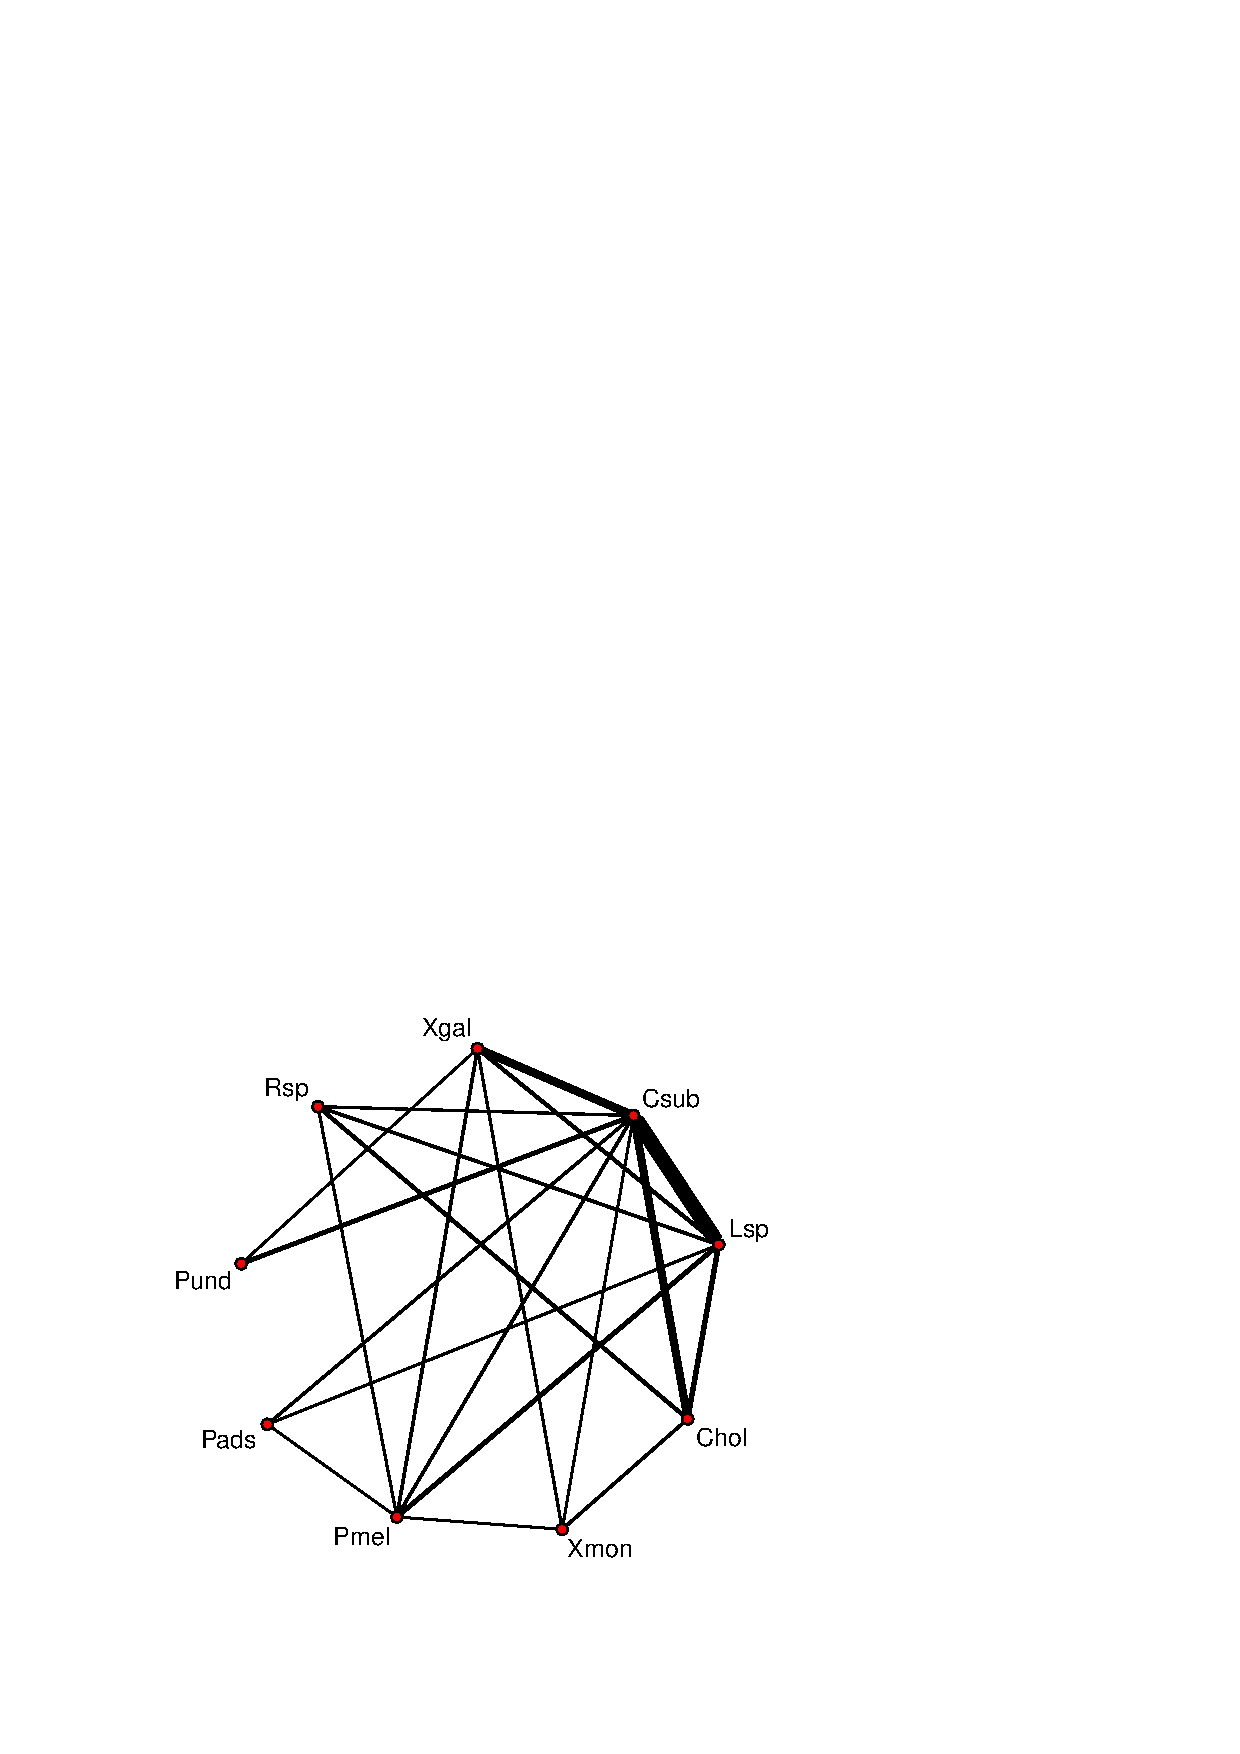
\includegraphics{LCO_analyses-018}

\newpage
\paragraph{}\textbf{Mean graphs for each genotype.}

\begin{Schunk}
\begin{Sinput}
> cor.l. = cor.l[garden == "ONC"]
> geno.A = A[garden == "ONC"]
> geno.A. = A.[garden == "ONC"]
> geno.net = list()
> for (i in (1:length(unique(geno.onc)))) {
+     x = cor.l.[geno.onc == unique(geno.onc)[i]]
+     geno.net[[i]] = x[[1]]
+     for (j in (2:length(x))) {
+         geno.net[[i]] = geno.net[[i]] + x[[j]]
+     }
+     geno.net[[i]] = geno.net[[i]]/length(x)
+ }
> names(geno.net) = unique(geno)
\end{Sinput}
\end{Schunk}

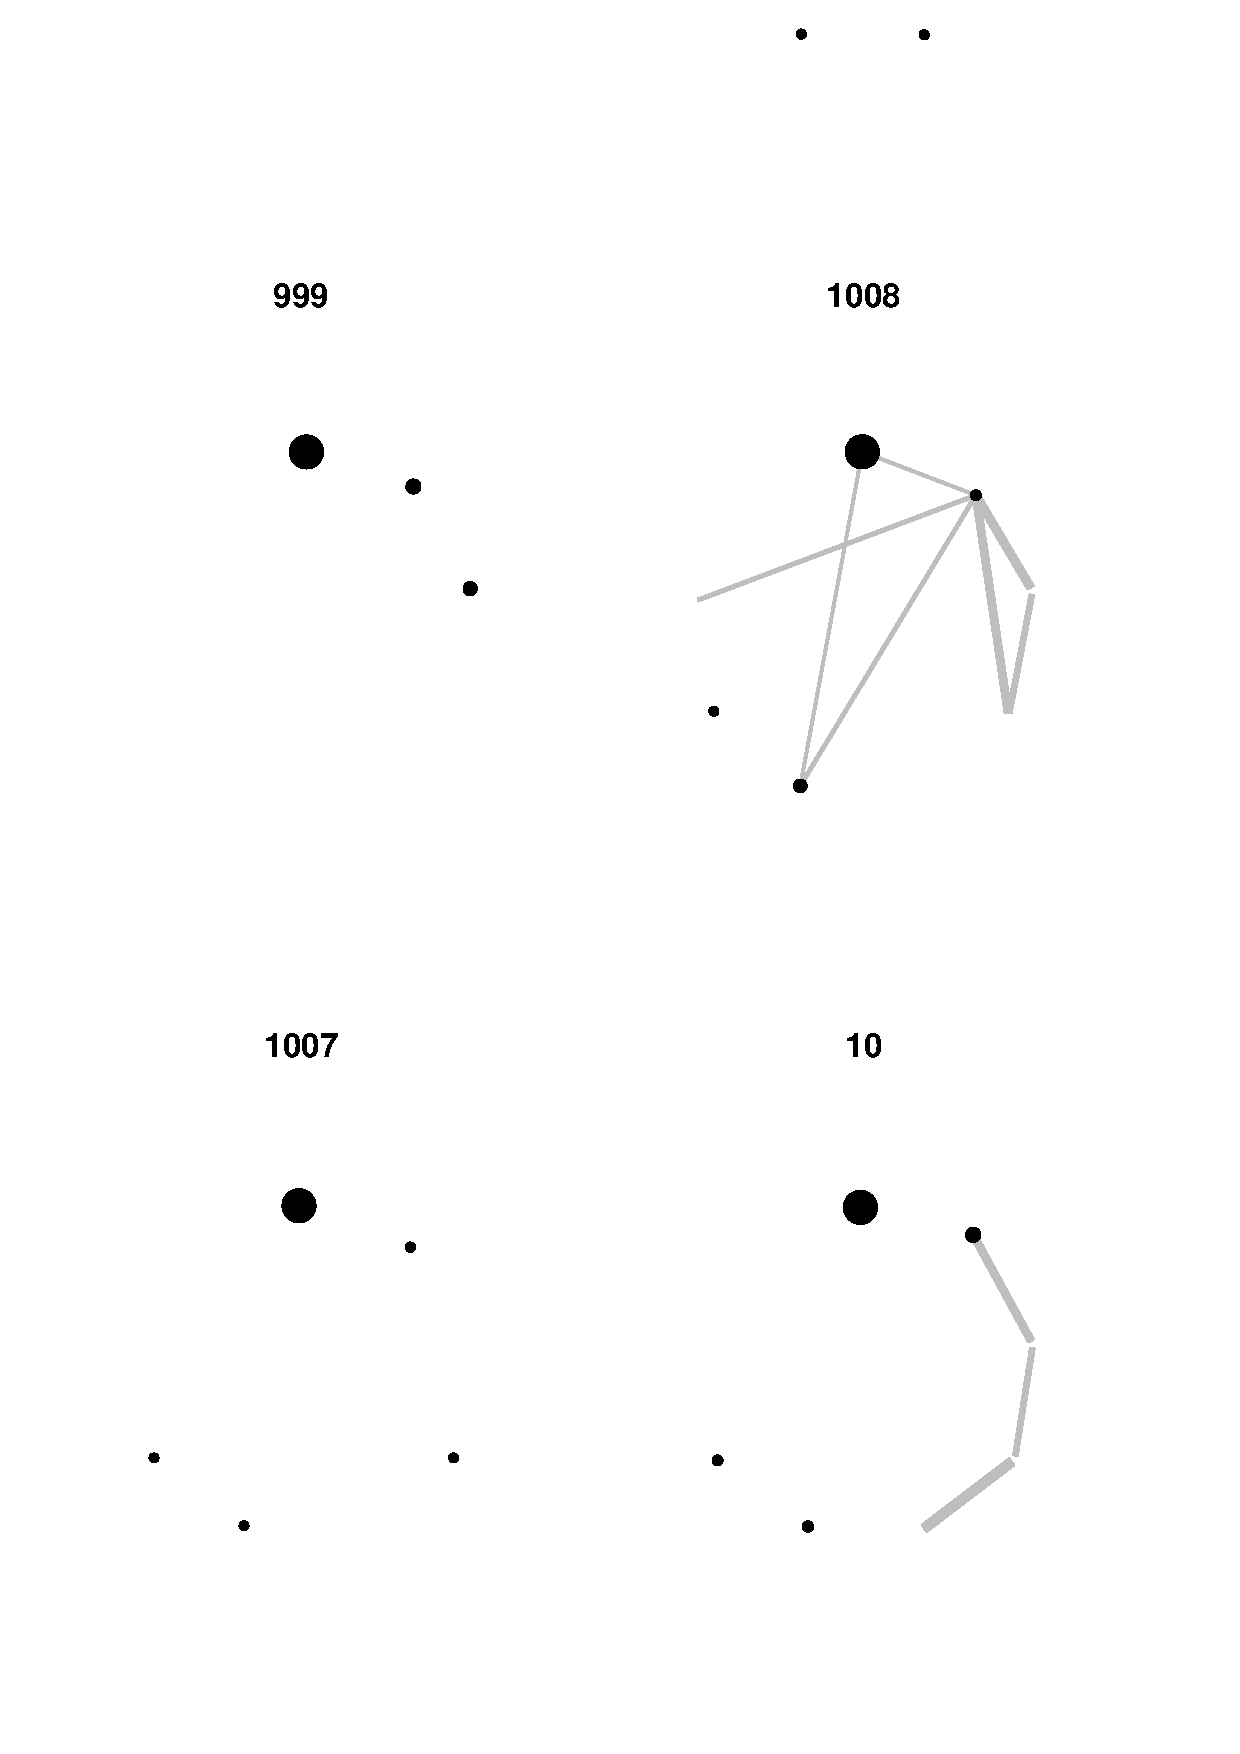
\includegraphics{LCO_analyses-020}

\newpage
\paragraph{}\textbf{ONC Network Statistics}
\begin{Schunk}
\begin{Sinput}
> par(mfrow = c(2, 2))
> bplot(geno.onc, n.onc, "Size")
> bplot(geno.onc, L.onc, "Number of Edges")
> bplot(geno.onc, C.onc, "Connectance")
> bplot(geno.onc, Cf.onc, "Centralization")
\end{Sinput}
\end{Schunk}
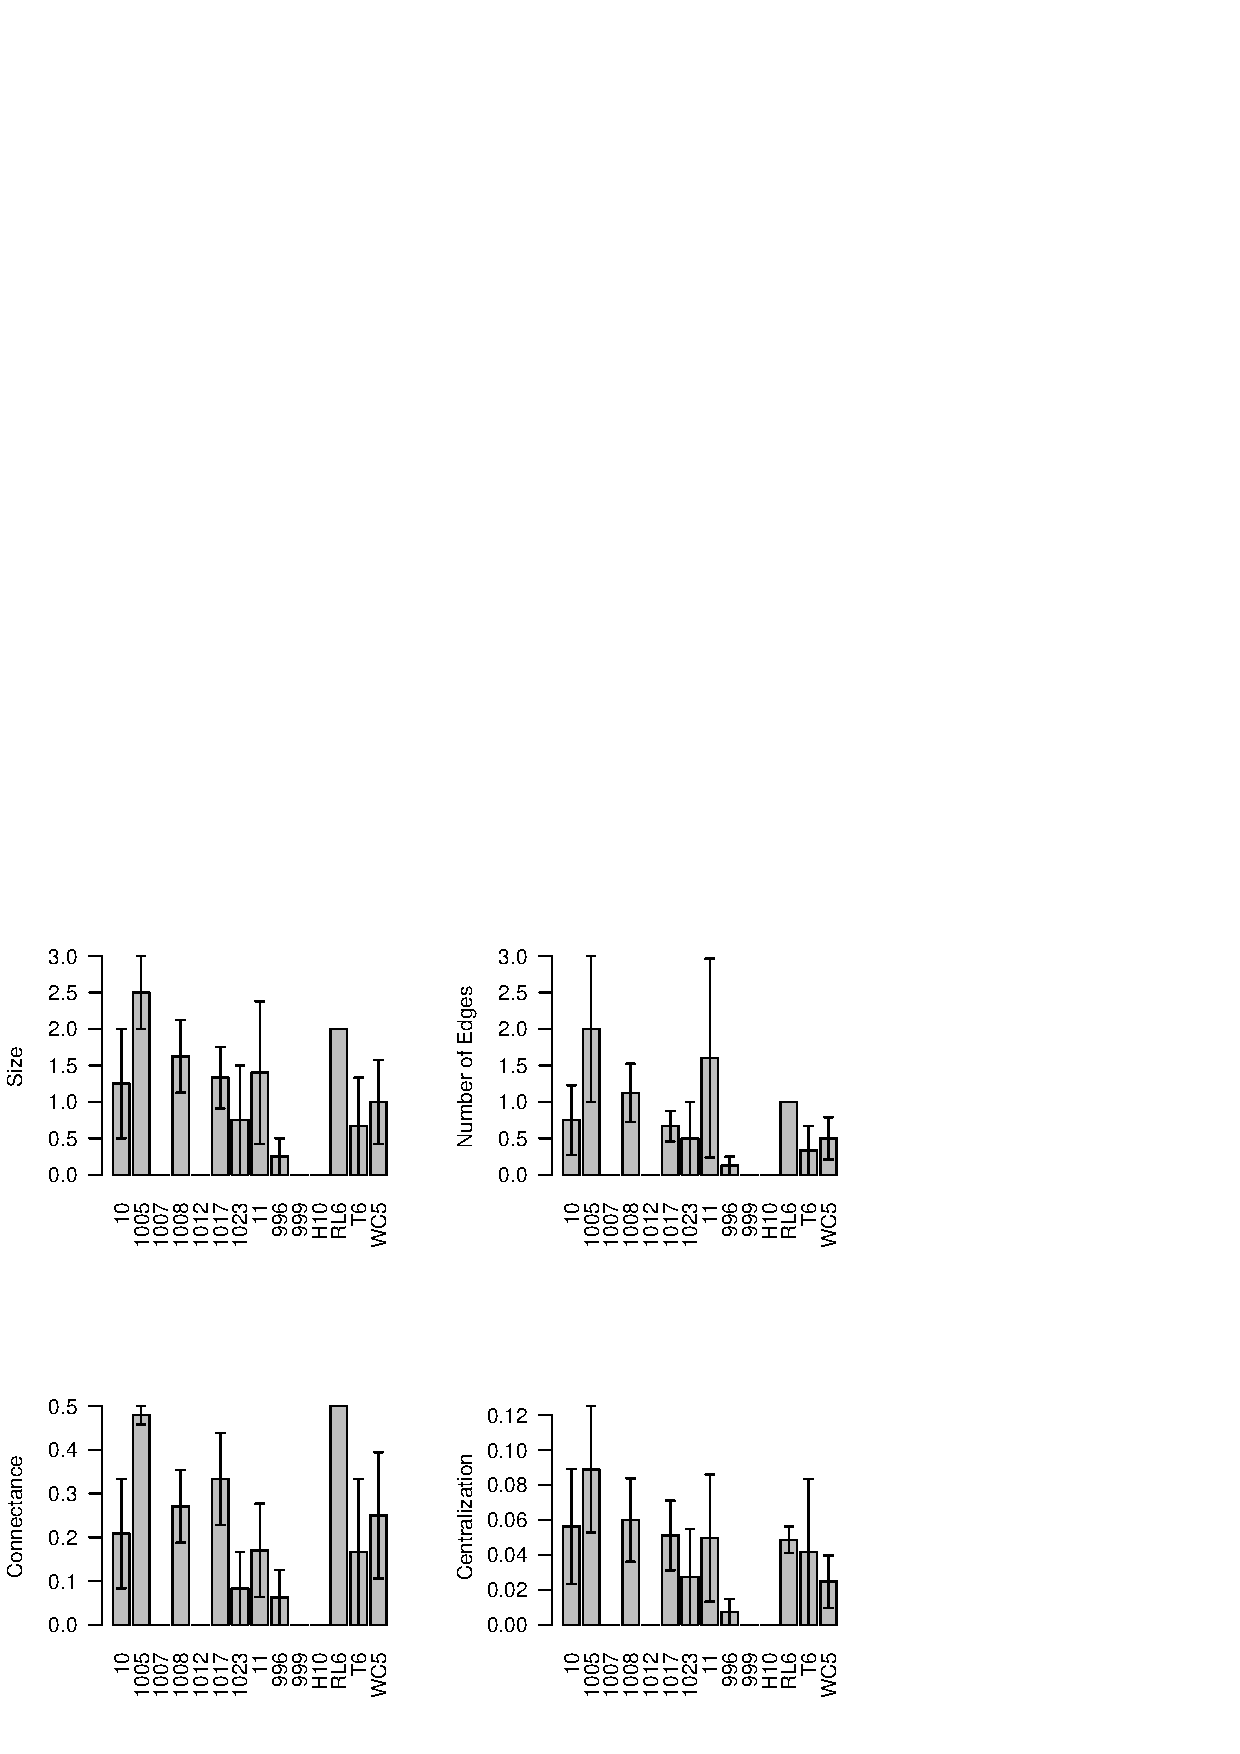
\includegraphics{LCO_analyses-021}

\newpage
\paragraph{}\textbf{PIT Network Statistics}

\begin{Schunk}
\begin{Sinput}
> par(mfrow = c(2, 2))
> bplot(geno.pit, n.pit, "Size")
> bplot(geno.pit, L.pit, "Number of Edges")
> bplot(geno.pit, C.pit, "Connectance")
> bplot(geno.pit, Cf.pit, "Centralization")
\end{Sinput}
\end{Schunk}
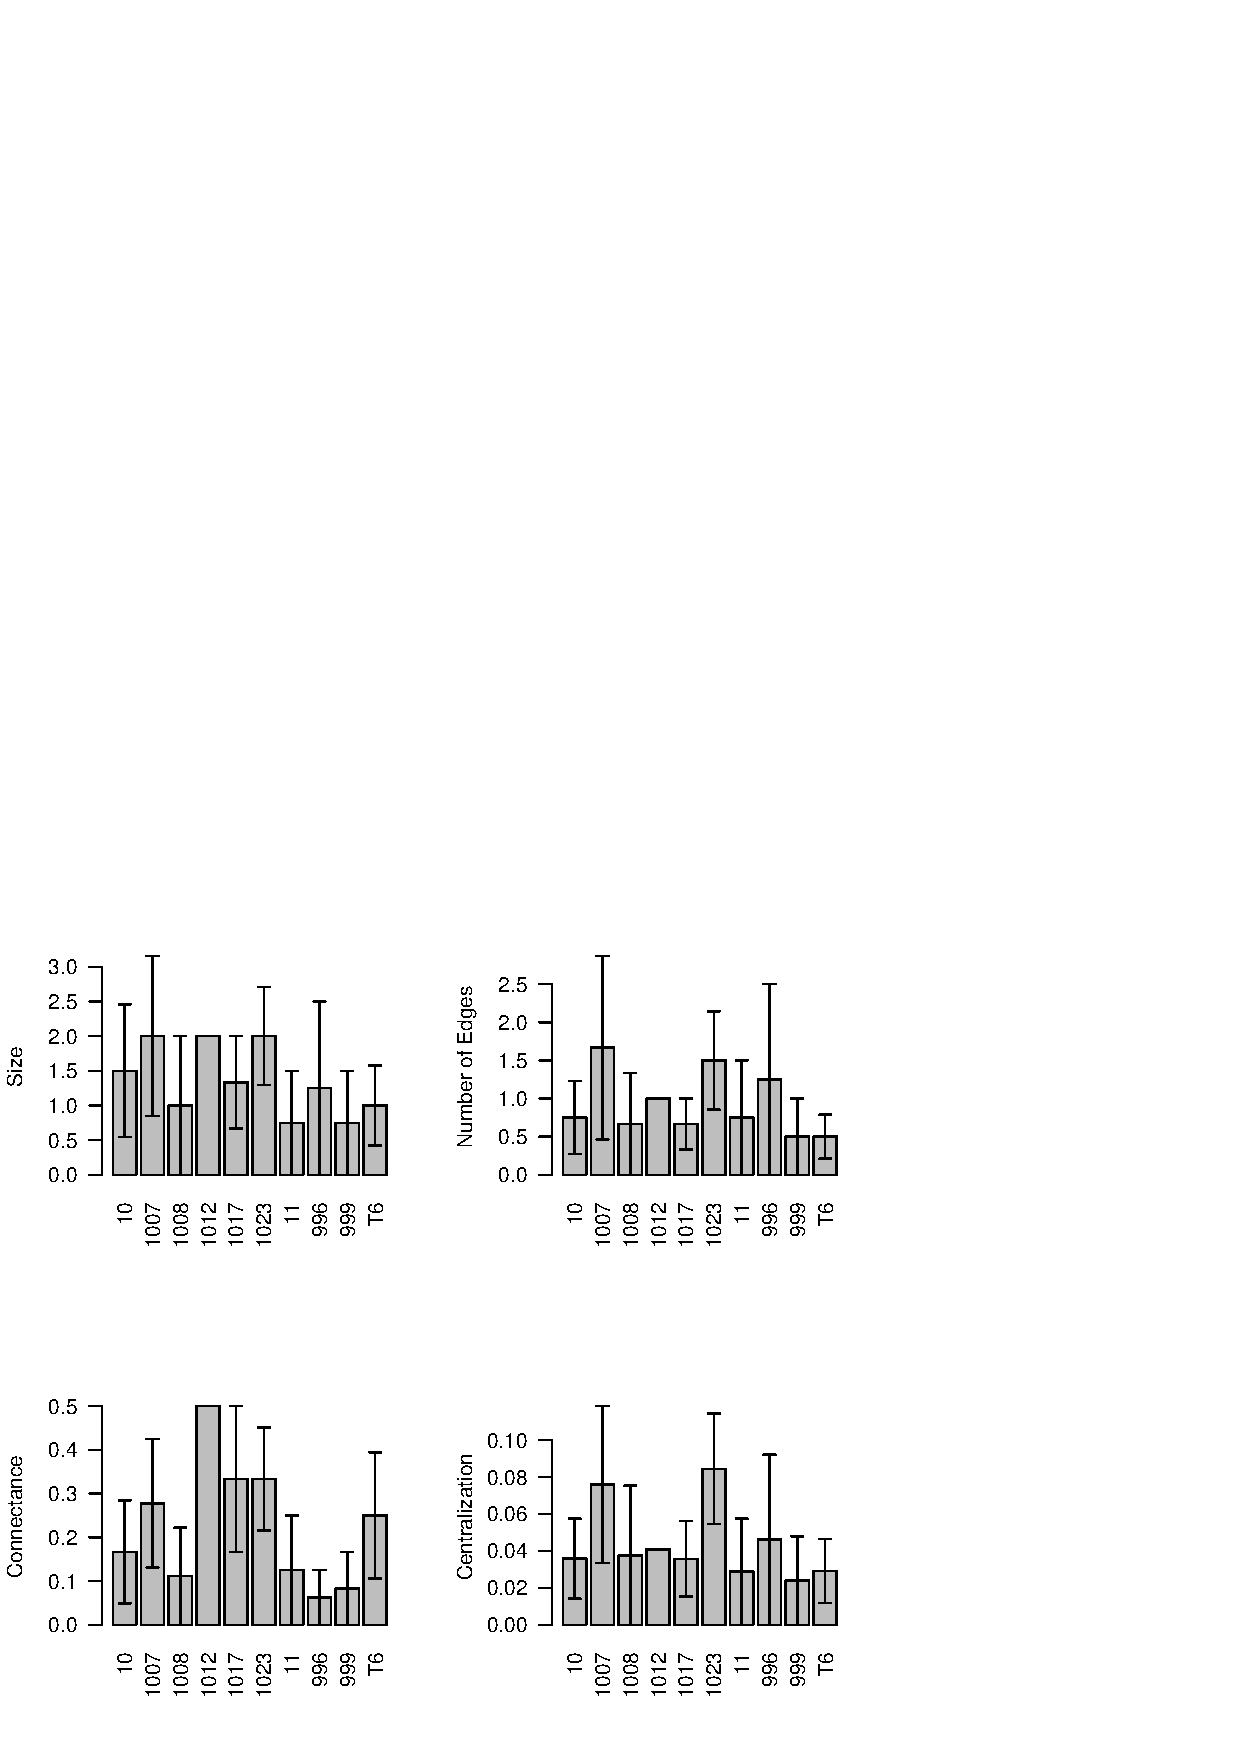
\includegraphics{LCO_analyses-022}

\end{document}  
